\documentclass[conference]{IEEEtran}
\IEEEoverridecommandlockouts

\usepackage{cite}
\usepackage{amsmath,amssymb,amsfonts}
\usepackage{algorithmic}
\usepackage{graphicx}
\usepackage{textcomp}
\usepackage{xcolor}
\usepackage{hyperref}

\begin{document}

\title{Know your enemy and know yourself}
% \subtitle{Detecting AI generated text with source model prediction}
\author{
  \IEEEauthorblockN{Bo-Yi Mao}
  \IEEEauthorblockA{
    \textit{Dept. of Computer Science} \\
    \textit{National Tsing-Hua University}\\
    Hsinchu, Taiwan
  }
  \and
  \IEEEauthorblockN{Aurick}
  \IEEEauthorblockA{
    \textit{Dept. of Computer Science} \\
    \textit{National Tsing-Hua University}\\
    Hsinchu, Taiwan
  }
  \and
  \IEEEauthorblockN{Kenneth}
  \IEEEauthorblockA{
    \textit{Dept. of Computer Science} \\
    \textit{National Tsing-Hua University}\\
    Hsinchu, Taiwan
  }
  \and
  \IEEEauthorblockN{Yi-Hsueh Chu}
  \IEEEauthorblockA{
    \textit{Dept. of Computer Science} \\
    \textit{National Tsing-Hua University}\\
    Hsinchu, Taiwan
  }
}

\maketitle

\section{Introduction}

With the recent boom of generative models and large language models (LLMs), their potential has enabled plagiarism in academic writing. The Detect AI Generated Text (DAIGT) competition hosted on Kaggle \cite{daigt} aims to identify and discriminate AI-generated essays to ensure fairness in the usage of LLMs.

Previous works mostly focus on improving training data quality and diversity and using larger and larger models. However, few have attempted to address the distribution difference of different language models. In this paper, we present our approach to detecting AI-generated text by predicting the source model used to generate the text. We explore various machine learning techniques and natural language processing (NLP) methods to achieve this goal. Our contributions include a comprehensive dataset of AI-generated and human-written texts, a detailed analysis of different models' performance, and insights into the features that distinguish AI-generated text from human-written text.

\section{Previous Works}

Transformer-based classification models often struggle to generalize from the PERSUADE corpus dataset to the private test dataset, frequently tending towards overfitting. As a result, many attempts have resulted in scores around 0.75, despite performing well on local validation. Consequently, many have found other approaches to tackling the problem.

One notable success from Bamba et al. \cite{1stplace} involved increasing both the diversity and size of the training dataset. Yhey achieved a significant improvement in accuracy by leveraging a diverse and extensive dataset. They utilized a combination of AI-generated and human-written texts, which helped in training robust models capable of distinguishing between the two, eventually winning the competition in first place, with a score of 0.988.

Another work from Day \cite{5thplace} used 500,000 documents from The Pile and another 500,000 plausible continuations generated with local LLMs, and resulted in a sizeable increase in accuracy; in fact, they submitted a DeBERTa-v3 LLM at a context length of 1024 tokens with scores of 0.96 for individual models and 0.963 for an ensemble. Compared to the models trained on the PERSUADE corpus, which scored around 0.75, this is a significant improvement.

However, Cozzolino \cite{6thplace} took a different approach by using synthetic features such as entropy, surprisal, and average word length. By merely focusing on these features, Cozzolino was able to achieve a competitive score in the DAIGT competition. As shown in Figure \ref{fig:cozzolino}, his method demonstrated that even without relying heavily on large datasets or complex models, it is possible to achieve good performance by carefully selecting and engineering features that capture the nuances of AI-generated text.

\begin{figure}[htbp]
  \centerline{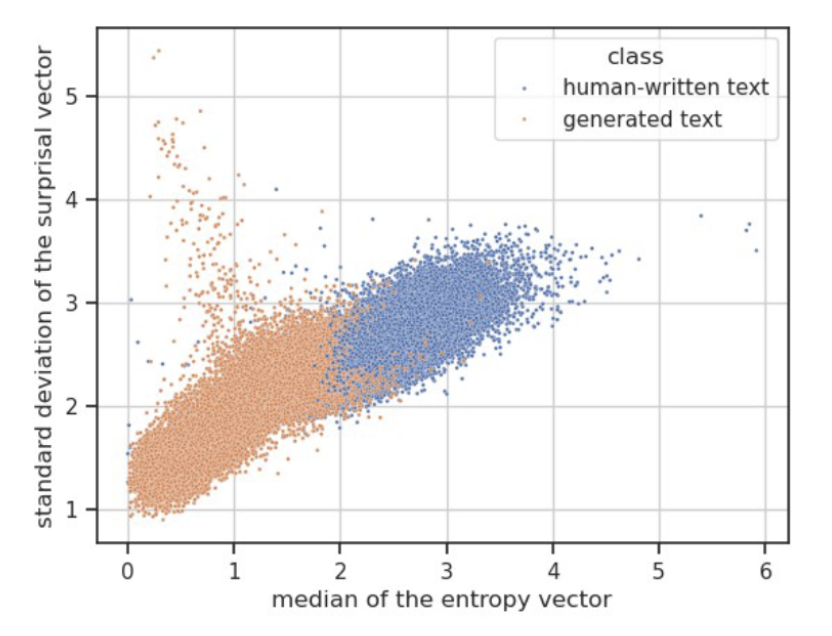
\includegraphics[width=\columnwidth]{figs/cozzolino.png}}
  \caption{Engineered features used by Davide Cozzolino \cite{6thplace} separates AI-generated text from human-written text well.}
  \label{fig:cozzolino}
\end{figure}

\section{Methodology}

Our methodology overall consists of three steps. First, the data is prepared and preprocessed ahead of time, published to Kaggle, and ready to be used. Second, certain representation learning models perform feature extraction on raw data. Finally, binary/multi-class classification is performed via various machine learning methods.

\subsection{Data Preparation}
\label{sec:data}

We collected training data from several sources \cite{persuade,mistral7btext,argugpt,daigtv4,fpeprocessed}, containing 87k AI-generated and 13k human-written essays, with prompts from PERSUADE, WECCL, TOEFL, and GRE corpus. The generated essays are generated from various models, including T5, LLaMA series, GPT series, Mistral7B, Claude, Falcon, T5, PaLM, and Cohere. The class distributions (AI-generated vs. human-written) are shown in Figure \ref{fig:class_dist}, and the distribution of source models is shown in Figure \ref{fig:source_dist}.

\begin{figure}[htbp]
  \centerline{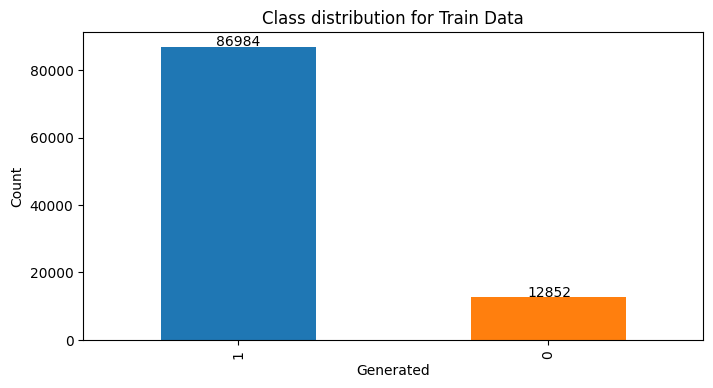
\includegraphics[width=\columnwidth]{figs/class_dist.png}}
  \caption{Class distribution of AI-generated and human-written essays}
  \label{fig:class_dist}
\end{figure}

\begin{figure}[htbp]
  \centerline{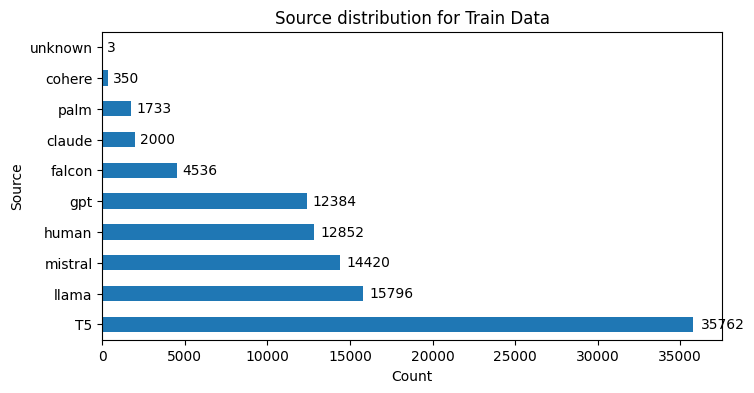
\includegraphics[width=\columnwidth]{figs/source_dist.png}}
  \caption{Distribution of source models}
  \label{fig:source_dist}
\end{figure}

\subsection{Text Tokenization}

\subsubsection{Byte Pair Encoding}

Byte Pair Encoding (BPE) is a subword tokenization algorithm that is widely used in NLP tasks. It works by iteratively merging the most frequent pair of bytes (or characters) in a given text corpus. Initially, every character in the text is treated as a separate token. The algorithm then finds the most frequent pair of adjacent tokens and merges them into a single token. This process is repeated until a predefined vocabulary size is reached or no more pairs can be merged.

The main advantage of BPE is that it can effectively handle rare and out-of-vocabulary words by breaking them down into smaller, more frequent subword units. This allows models to represent and generate words that were not seen during training, improving their ability to generalize to new text.

\subsubsection{AutoTokenizer}

AutoTokenizer is a convenience tool provided by Hugging Face. It can automatically select a tokenizer which fits the model the most. Besides, it also provides a uniformed API, so that we can use different tokenizers with the same code. For example, we use AutoTokenizer in the DeBERTa model structure by calling: \texttt{AutoTokenizer.from\linebreak\_pretrained("microsoft/deberta-v3-base")}.

\subsection{Feature Extraction}

\subsubsection{TF-IDF}

Term Frequency-Inverse Document Frequency (TF-IDF) is a popular technique for document vectorization, which is proven to be useful in various text classification tasks. The TF-IDF vector is calculated as follows:
\begin{gather}
  \text{TF}(t, d) = \frac{n_{t, d}}{\sum_{t' \in d} n_{t', d}} \\
  \text{IDF}(t) = \log \frac{|D|}{|{d \in D : t \in d}|} \\
  \text{TF-IDF}(t, d) = \text{TF}(t, d) \times \text{IDF}(t)
\end{gather}

where $D$ is the set of all documents, $n_{t, d}$ is the number of occurrences of term $t$ in document $d$, $\text{TF}(t, d)$ is the term frequency of term $t$ in document $d$, and $\text{IDF}(t)$ is the inverse document frequency of term $t$ in the corpus. The TF-IDF vector is then normalized to have unit norm.

We use TF-IDF to extract features from the text data, which are then used as input to the classifier. The TF-IDF vectorizer is trained on the training data and used to transform both the training and test data.

\subsubsection{Entropy-based Features}
% (Aurick, 6th place sol, entropy and surprisal-based features)

Huang et al. \cite{huang2023gpt} proposed GPT-based Arithmetic Coding (GPT-AC) to encode text data with entropy-based compressor that involves the GPT model. Drawing inspiration from this work, Cozzolino \cite{6thplace} incorporated the following features into the classifier:
\begin{itemize}
  \item \textbf{Entropy:} The expected value of the information contained in each token, indicating the randomness of the text.
  \item \textbf{Surprisal:} The negative log-likelihood of each token, indicating the unexpectedness of the text.
  \item \textbf{Average word length:} The average length of the words in the text data, indicating the complexity of the text.
\end{itemize}

To use the entropy and surprisal-based features, however, Cozzolino utilized the statistical properties of the data, including median, standard deviation, mean, and quantiles. These features were then used to train a SVM classifier, which achieved a competitive score in the DAIGT competition.

\subsubsection{LLM Embedding}
\label{sec:llm_embedding}

LLMs are known for their ability to generate high-quality text, but they can also be used to extract features from text data. We fine-tuned both Mistral7B and DeBERTa using our dataset, allowing it to react to subtle stylistic and structural cues common in synthetic text.

Mistral7B is a 7-billion-parameter language model engineered by the Mistral AI team. Our method makes use of the model's ability to analyse textual properties and discover patterns that distinguish human-written content from machine-generated language \cite{mistral7b}.

DeBERTa is a state-of-the-art transformer-based model developed by Microsoft. It introduces two key innovations, which are Disentangled Attention Mechanism and Enhanced Masked Encoding. The former mechanism enables the model to focus more efficiently on semantic relationships without being overly constrained by word order. The latter skill improves its ability to model dependencies across long sequences and better capture the contextual nuances of text \cite{deberta}.

After we get the output from LLMs, a mean pooling is implemented to extract a general feature. Filtering out the valid tokens with \texttt{attention\_mask}, those tokens are summed and divided with the number of valid tokens to get the mean embedding. At last, passing over the \texttt{mlp\_head}, a sequence of fully-connected layers, will it be transformed into a feature vector.

\subsection{Classification}

\subsubsection{Traditional Machine Learning}
\label{sec:traditional_ml}

Drawn from the top solutions in the competition, we experimented with an ensemble of classifiers, including linear classifiers, multinomial naive Bayes, and LightGBM. The hyperparameters are the same as the original solution. The final prediction is made by weighted voting of the three classifiers:
\begin{equation}
  \hat{y} = 0.1 \times \hat{y}_{\text{Bayes}} + 0.45 \times \hat{y}_{\text{linear}} + 0.45 \times \hat{y}_{\text{LGBM}}
\end{equation}

To experiment with our hypothesis for source model prediction, we set up two classification tasks: binary classification (AI-generated or human-written) and multi-class classification (source model prediction). For binary classification, each classifier is trained to distinguish between AI-generated and human-written essays. For multi-class classification, each classifier is trained to predict the source model of the AI-generated essays.

Specially for multi-class classification, we also experimented with different class weights to balance the class distribution. The vanilla class weights are calculated as the inverse of the class frequency in the training data, and the hyperparameter \texttt{human\_factor} is multiplied to the class weights of the human-written class. The class weights are then used in the training of the classifier.

% (Aurick, SVM, short explanation)

\subsubsection{Deep Learning}

With the embedding vector generated as described in Section \ref{sec:llm_embedding}, we can use a deep learning model to classify the text. We experimented with simple feed-forward neural networks, getting promising results. The model is trained for 5 epochs and evaluated on the validation set with the ROC-AUC score.

\subsubsection{Ensemble}

The ensemble approach involved a weighted averaging of probabilities generated by individual classifiers. This allowed the models to compensate for each other's weaknesses and collectively improve accuracy. Beside using different model type, different training data can also be used to train the model.

\section{Experiments}

\subsection{Effect of Source Model Prediction}

We hypothesized that predicting the source model of the AI-generated text could help distinguish between AI-generated and human-written text. To test this hypothesis, we used BPE tokenization, TF-IDF feature extraction, and the ensemble classifier described in Section \ref{sec:traditional_ml} to predict the source model of the AI-generated essays. The results are shown in Table \ref{tab:multiclass} and plotted in Figure \ref{fig:multiclass}, with the dotted line indicating the baseline accuracy of binary classification.

As shown, the accuracy of multi-class classification is generally higher than that of binary classification. This suggests that predicting the source model of the AI-generated text does help distinguish between AI-generated and human-written text. The best accuracy is achieved with \texttt{human\_factor}=$3 \times 10^4$, being about 20\% higher than the baseline accuracy of binary classification.

Note that the accuracy for public and private scores differs significantly and consistently across different class weights. This suggests that the distribution of source models in the public and private test data is different, which may affect the generalization of the classifier. As stated in many previous works, the importance of training data diversity and quality is crucial for the generalization of the model, and our observation is consistent with this finding.

\begin{table}[htbp]
  \centering
  \caption{Effect of class weights on multi-class classification accuracy}
  \label{tab:multiclass}
  \begin{tabular}{rrr}
    \hline
    \textbf{\texttt{human\_factor}} & \textbf{Private Score} & \textbf{Public Score} \\
    \hline
    $0$ & 0.770701 & 0.920051 \\
    $1 \times 10^{-3}$ & 0.760378 & 0.919360 \\
    $1 \times 10^{-2}$ & 0.736073 & 0.897525 \\
    $3 \times 10^{-2}$ & 0.709871 & 0.880807 \\
    $1 \times 10^{-1}$ & 0.701310 & 0.873958 \\
    $5 \times 10^{-1}$ & 0.706552 & 0.883646 \\
    $1 \times 10^{0}$ & 0.697281 & 0.881103 \\
    $5 \times 10^{0}$ & 0.647095 & 0.866519 \\
    $1 \times 10^{1}$ & 0.636825 & 0.862602 \\
    $3 \times 10^{1}$ & 0.638540 & 0.872659 \\
    $5 \times 10^{1}$ & 0.652778 & 0.876469 \\
    $1 \times 10^{2}$ & 0.681232 & 0.884198 \\
    $3 \times 10^{2}$ & 0.704799 & 0.890483 \\
    $1 \times 10^{3}$ & 0.724823 & 0.902500 \\
    $3 \times 10^{3}$ & 0.752475 & 0.910431 \\
    $1 \times 10^{4}$ & 0.777595 & 0.915113 \\
    $3 \times 10^{4}$ & 0.807771 & 0.912862 \\
    $1 \times 10^{5}$ & 0.782545 & 0.898491 \\
    $3 \times 10^{5}$ & 0.777071 & 0.889535 \\
    $1 \times 10^{6}$ & 0.767274 & 0.887141 \\
    $3 \times 10^{6}$ & 0.748232 & 0.872659 \\
    $1 \times 10^{7}$ & 0.734994 & 0.864930 \\
    \hline
    Baseline: binary classification & 0.665908 & 0.891065 \\
    \hline
  \end{tabular}
\end{table}

\begin{figure}[htbp]
  \centerline{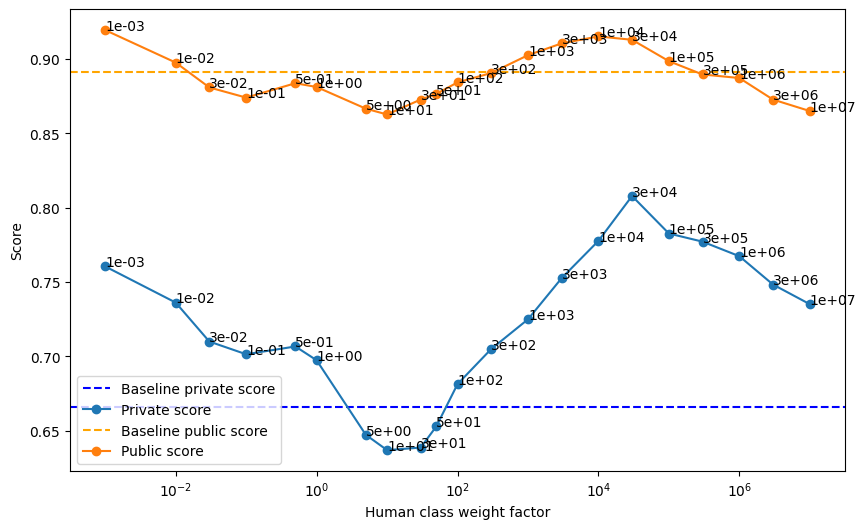
\includegraphics[width=\columnwidth]{figs/multiclass.png}}
  \caption{Effect of class weights on multi-class classification accuracy}
  \label{fig:multiclass}
\end{figure}

\subsection{Submission Results}

As the DAIGT competition is a code competition, we have to submit our code to Kaggle for evaluation. We have tested various models and hyperparameters, with some of the best results shown in Table \ref{tab:models}. The best model we have found is\dots

\begin{table*}[htbp]
  \centering
  \caption{Tested models and datasets, and their respective accuracies}
  \label{tab:models}
  \begin{tabular}{p{1.8cm}p{1.5cm}p{2.3cm}p{2.8cm}p{3.6cm}p{1.6cm}p{1.6cm}}
    \hline
    \textbf{Training Set} & \textbf{Tokenizer} & \textbf{Feature Extractor} & \textbf{Classifier} & \textbf{Hyperparameters} & \textbf{Private Score} & \textbf{Public Score} \\
    \hline
    Ours & BPE & TF-IDF & Multi-class ensemble & \texttt{human\_factor}=$3 \times 10^4$ & 0.807771 & 0.912862 \\
    Ours & BPE & TF-IDF & Multi-class ensemble & \texttt{human\_factor}=$1 \times 10^5$ & 0.782545 & 0.898491 \\
    Ours & BPE & TF-IDF & Multi-class ensemble & \texttt{human\_factor}=$0$ & 0.770701 & 0.920051 \\
    Ours & BPE & TF-IDF & Multi-class ensemble & \texttt{human\_factor}=$1 \times 10^{-3}$ & 0.760378 & 0.919360 \\
    Ours & BPE & TF-IDF & Binary ensemble & \texttt{tokenizer\_lower}=\texttt{False} & 0.665908 & 0.891152 \\
    Ours & BPE & TF-IDF & Binary ensemble & \texttt{tokenizer\_lower}=\texttt{True} & 0.658713 & 0.894109 \\

    Ours & Mistral & Mistral7b & Mistral7b & - & 0.702772 & 0.854477 \\
    Base & Mistral & Mistral7b & Mistral7b & - & 0.53 & 0.54 \\
    \hline
  \end{tabular}

  \vspace{0.5cm}

  \begin{tabular}{ll}
    \hline
    \textbf{Classifier} & \textbf{Description} \\
    \hline
    Multi-class ensemble & Ensemble of linear classifier, multinomial naive bayes, and LightGBM, classifying source model. \\
    Binary ensemble & Ensemble of linear classifier, multinomial naive bayes, and LightGBM, with binary classification. \\
    Mistral7b & Mistral7b model finetuned for binary classification. \\
    \hline
  \end{tabular}

  \vspace{0.5cm}

  \begin{tabular}{ll}
    \hline
    \textbf{Training Set} & \textbf{Description} \\
    \hline
    Ours & Our dataset, as described in Section \ref{sec:data}. \\
    Base & The base dataset provided by the competition. \\
    \hline
  \end{tabular}
\end{table*}

\section{Conclusion}

Our work demonstrates the importance of source model prediction in detecting AI-generated text. By predicting the source model of the AI-generated text, we can outperform the baseline accuracy of binary classification. This suggests that the distribution of source models is an important factor in distinguishing between AI-generated and human-written text.

However, the accuracy of the classifier is still limited by the quality and diversity of the training data. As shown by Cozzolino \cite{6thplace}, even with simple features, it is possible to achieve good performance by carefully selecting and engineering features that capture the nuances of AI-generated text. With more diverse training data and better feature extraction techniques, and by leveraging the distribution of source models, we can expect much better results in detecting AI-generated text.

\section{Data and Code Availability}

Our own dataset is available on Kaggle at \url{https://www.kaggle.com/datasets/dogeon188/daigt-datamix}. The code for our experiments is available on GitHub at \url{https://github.com/Dogeon188/NLP-term-daigt}.

\bibliographystyle{IEEEtran}
\bibliography{refs}

\end{document}